%
% kernbild.tex -- Kern und Bild einer Matrix
%
% (c) 2021 Prof Dr Andreas Müller, OST Ostschweizer Fachhochschule
%
\documentclass[tikz]{standalone}
\usepackage{amsmath}
\usepackage{times}
\usepackage{txfonts}
\usepackage{pgfplots}
\usepackage{csvsimple}
\usetikzlibrary{arrows,intersections,math}
\begin{document}
\def\skala{1}
\definecolor{darkgreen}{rgb}{0,0.4,0}
\definecolor{turqoise}{rgb}{0,0.3,0.6}
\begin{tikzpicture}[>=latex,thick,scale=\skala]

\begin{scope}[xshift=-3.5cm]
\node at (0,0) {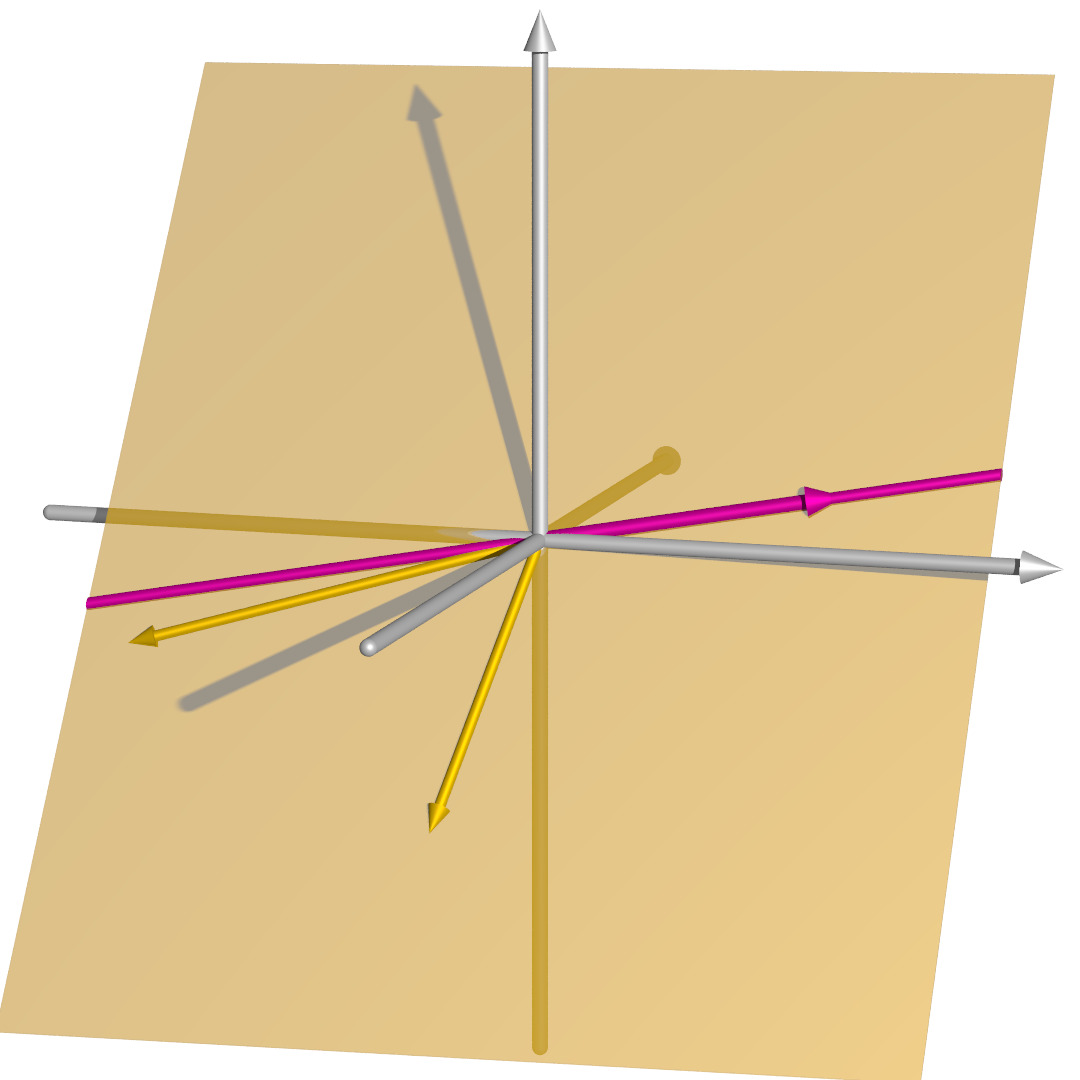
\includegraphics[width=6.8cm]{bild2.jpg}};

\fill[color=white,opacity=0.8] (-3,-2.75) rectangle (-2,-2.3);
\node[color=orange] at (-2.5,-2.5) {$\mathcal{J}^1(A)$};
\node at (3.3,0) {$x_1$};
\node at (0.3,3.2) {$x_3$};
\node[color=purple] at (2.3,0.6) [rotate=8] {$\mathcal{J}^2(A)$};
\end{scope}

\begin{scope}[xshift=3.5cm]
\node at (0,0) {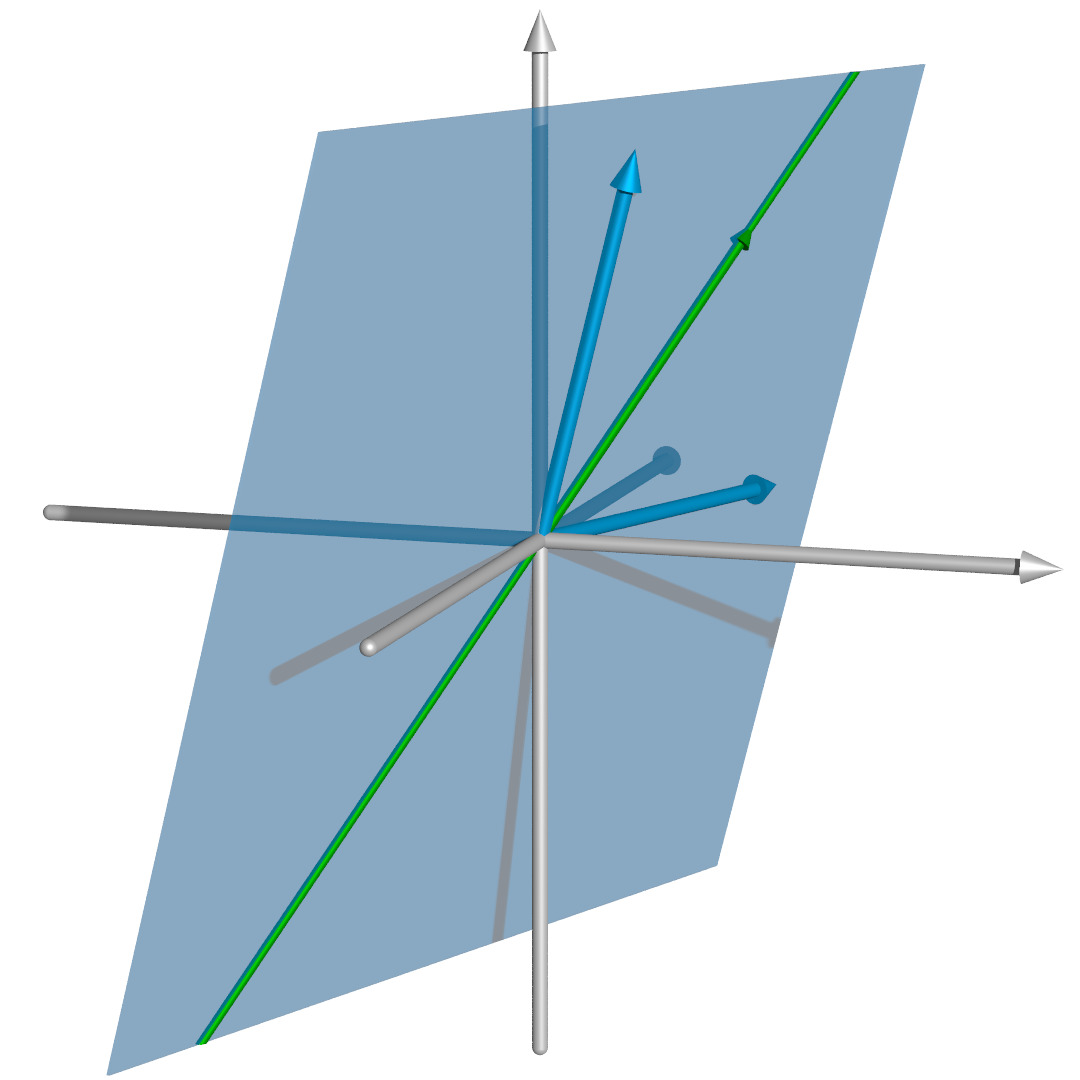
\includegraphics[width=6.8cm]{kern2.jpg}};
\node[color=darkgreen] at (1.8,2.2) [rotate=58] {$\mathcal{K}^1(A)$};
\fill[color=white,opacity=0.8] (-1.5,0.8) rectangle (-0.5,1.2);
\node[color=turqoise] at (-1,1) {$\mathcal{K}^2(A)$};
\node at (3.3,0) {$x_1$};
\node at (0.3,3.2) {$x_3$};
\end{scope}

\end{tikzpicture}
\end{document}

